Systematic literature review was conducted as a purpose to gain an overview of the current state of source code plagiarism research. We mainly focus on methods applied in this review, to find consensus about what is held as a well-performing approach to plagiarism detection. Our review consists six key steps that follows the structure of systematic review \cite{AGCSLRIS2010}: 1) purpose, 2) details of search, 3) inclusion criteria, 4) exclusion criteria, 5) information extraction and 6) analysis. To easily conduct the review we used a web service to gather the articles.


The database that was utilized to query research papers is called \emph{Scopus\footnote{\url{https://www.scopus.com/}}}, which is a service containing peer-reviewed scientific literature. It allows users to search scientific articles by matching \eg titles, abstracts or keywords to user-defined query. The service itself maintains links to articles which are published under for example \emph{ACM (Association for Computing Machinery)} and \emph{IEEE (Institute of Electrical and Electronics Engineers)}, both of these being major computer science releases. 

Following subchapters describe how the review was conducted and what kind of results were found. We first form a categorization between studies to gain overview of the methods that are applied, then we extract statistics about data sets used in studies, and finally show the various methods that are applied to detect plagiarism. 

\subsection{Methodology}

Querying Scopus can be done in a similar way as querying databases in SQL-like languages. The query used inside Scopus as inclusion step was following
\begin{verbatim}
TITLE-ABS-KEY (("plagiarism" OR "authorship identification")  
                AND "source code") 
AND  (LIMIT-TO (SUBJAREA,"COMP"))
\end{verbatim}

\noindent
Above query translates to searching for articles which title, abstract or keywords contains the word \emph{plagiarism} or \emph{authorship identification} and the term \emph{source code}. These keywords were chosen in order to find articles which study the problem of plagiarism finding from source code either in general terms, or by utilizing authorship identification techniques. Finally, the query limits the area of study to computer science publications to find relevant methods for this thesis. 

The total number of articles gathered by querying Scopus in the inclusive search part of the literature review was 187, and the date when the query was done was 7th of February 2018. The distribution of studies per year can be seen in the following plot.

\begin{figure}[ht]
\centering
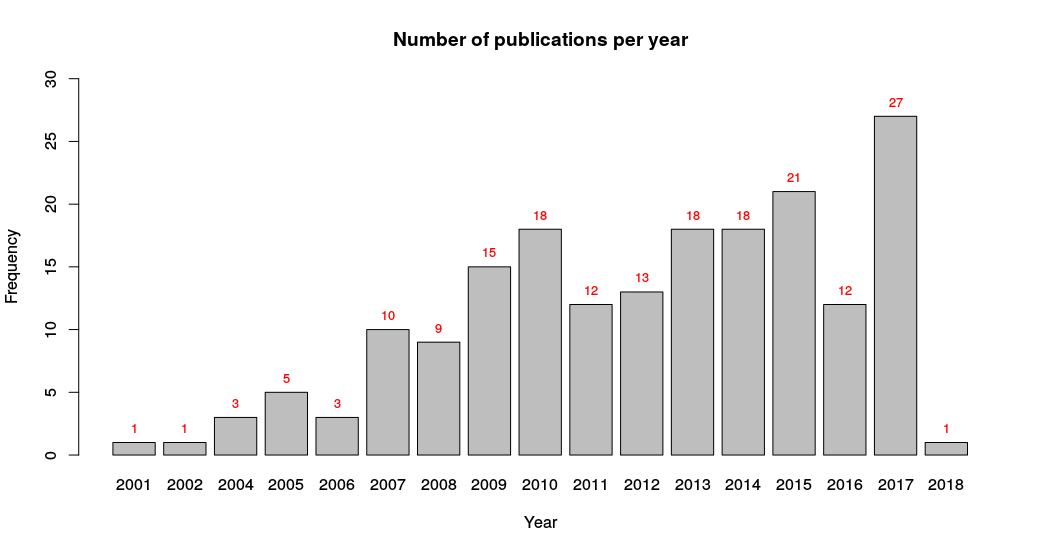
\includegraphics[width=\textwidth]{plots/Rplot.png}
\caption{Results of inclusion phase}
\end{figure}

After the inclusive search, we performed exclusion phase. This was done by filtering out manually all articles that were any of the following types: a review of certain aspect of source code plagiarism e.g. student motives behind plagiarism, an improvement to some pre-existing algorithm\footnote{In this context meaning algorithmic speedup}, plugin to online learning management systems, application to competition where the used method wasn't explained, study that used either byte-level information or information gathered during running the program, hashing techniques\footnote{Using the size of compression as a metric}, system review which didn't address the method and theses. Beside these attributes, articles needed to also test their proposed method in some way and the amount of documents in experiment phase needed to be larger than two. The reason for adding this as a limiting factor was to gather studies that used test sets to evaluate the performance of their model.

The final number of articles after exclusion, and which are inspected more carefully in this systematic literature review is 32. From the set of 32 studies, we look answers for following questions: \emph{how plagiarism can be detected from source code}, \emph{what are possible features that can be derived from source code} and \emph{how can one identify the author of a given source code}. We start first by categorizing the articles by their themes to see what kind of different approaches there are to deal with the problem of plagiarism detection. After the initial classification, we summarize statistics about data and briefly explain the methods.


\subsection{Categorization}

The naïve categorization between articles can be done in a similar fashion as was used by the query; dividing papers either to be about the detection of plagiarism or identifying the author of a given source code. However, as authorship identifying can also work as a way to detect plagiarism by verifying the author, we use the following high-level split visible in a table \ref{table-highcateq} where similarity detection is used as a second major category to avoid overlap.

\begin{table}[ht]
    \caption{Papers divided into two high-level categories}
    \label{table-highcateq}
    \centering
    \begin{tabular}{ | c | c | }
        
        \hline
        {\bf Similarity detection} & {\bf Authorship identification} \\ \hline
    
        \cite{AFAPLI2015, LICD2010, AASCPD2012} & \cite{SCAANN2017, ABEC2014, CAPSCAP2014}   \\
        \cite{Heblikar2015NormalizationBS, USCR2014, AIR2015} &  \cite{SCANG2007, EJPFSAI2004, ACSBPD2012}\\
        \cite{OTIOLSS2015, BUAA2009, ramirez2015high} &  \cite{APASCAI2007, UCMHGAAI2007, ESHPFSCAC2008}\\
        \cite{Ohmann2015, TBCFPD2012, Fu2017WASTKAW} &  \cite{AIRTSCAA2009, TSUDIJSCAI2011, DNNSCAI2013} \\
        \cite{ASTMLPD2013, AAPSCDPTK2013, CPDPPD2013}    & \cite{SCAIUFL2013, SDNAIJSP2015, AISC2017} \\
        \cite{PACASCD2005, RCISCP2017} &  \\ \hline
        {\bf Number of papers} & {\bf Number of papers} \\ \hline
        17 & 15 \\ \hline
    \end{tabular}
\end{table}

\noindent
Even though the articles are quite evenly divided in table \ref{table-highcateq}, these high-level groups are still too large to get a good overview of various methods. Thus we continue to categorize both groups into smaller atomic categorization, which reveals differences between and inside of them.  

Similarity detection in itself can be further divided into at least two general categories based on the current tools \cite{RSCAD2016}: attribute and structure. Then naturally, as authorship identification uses features derived directly from the source code too, we can use the same categorization to authorship identification studies. However, there are more finer categorizations that define the studies better based on the features they use, and thus we propose the following categories and their abbreviations: \emph{attribute counting (AC)}, \emph{segment matching (SM)}, \emph{n-gram (NG-STR)}, \emph{tree-based (TREE-STR)} and lastly \emph{hybrid approaches (HYB-STR)}. If a category has no studies under it, we leave the category out from the upcoming tables. These categories can be summarized briefly as following and are similar to categories identified from other plagiarism detection studies by Ali \etal \cite{OCPOCP2011}. 

\paragraph{Attribute counting}
Studies utilizing countable statistics, often referred as \emph{metrics}, that are gathered from source codes. This includes any features derived directly from source code like amount of words per line, number of lines per source code and number of keywords. For example the first two programs in appendix \ref{appendix:programs} represented as metrics is seen below.

\begin{table}[ht]
    \centering
    \begin{tabular}{|c|c|c|} \hline
        \textbf{Line count} & \textbf{Empty spaces} & \textbf{Semicolon count}\\ \hline
         10 & 1 & 5 \\ \hline
         8 & 1 & 3\\ \hline
    \end{tabular}
    \caption{Two sample programs represented as metrics}
    \label{tab:my_label}
\end{table}

\paragraph{Segment matching}
Considers two source codes as two strings and counts maximum match between them i.e. the longest common subsequence. These problems are also known as string matching problems, where one of the most famous algorithms is \emph{Greedy String Tiling} introduced early in \cite{SSGST1993}. As an example, statements \texttt{int a = 2;} and \texttt{int b = 2;} share 75\% of the character sequences and these matching sequences are: "\texttt{int}" and "\texttt{= 2;}". We also count all string similarity measures like string edit distances  to this category.

\paragraph{$N$-gram}
Treating the source code as a string and splitting it using a sliding window where the window size is the value of $n$ and the window traverses on either word or character level. This forms the vocabulary of the source code which is then transformed into occurrences of particular terms that are present, thus ultimately creating a vector representation of the source code. For example the statement \texttt{int a = 2} could be transformed into following word level 2-tuples using two as the value of $n$ (bigram). The first value of the following tuples is the $n$-gram extracted and the second value is the frequency: (\texttt{int a}, 1), (\texttt{a =}, 1), (\texttt{= 2}, 1). 

\paragraph{Tree-based}
Constructing a tree presentation from the source code, that captures the structure. For example diagram \ref{diag-parse} captures the structure of a simple assignment in parse tree, and one could compare \eg nodes of trees to define a similarity. The generation of a tree presentation usually requires some kind of parser being a very language specific feature. The inspection of a generated tree can be done with tree traversal methods for example using recursive functions. 

\paragraph{Hybrid}
Combines the usage of tree structure with $n$-gram representation. For example it can be a method which traverses abstract syntax tree, prints it and generates $n$-gram representation from the output.
\\\\
Now we can make a subcategorization for previously mentioned high-level classes; similarity detection and for authorship identification. Results for similarity detection studies can be seen from the following table, where most of them use structural features, indicated by the STR-ending. Many articles also tends to use $n$-grams to represent the source code.

\pagebreak

\begin{table}[ht]
    \caption{Subgroups and sizes of similarity detection studies}
    \label{table-sdstudies}
    \centering
    \begin{tabular}{ | c | c | c | c | c |}
        
        \hline
        {\bf AC} & {\bf SM} & {\bf NG-STR} & {\bf AST-STR} & {\bf HYB-STR} \\ \hline
        \cite{PACASCD2005} & 
        \cite{LICD2010, ASTMLPD2013} & 
        \cite{AASCPD2012, USCR2014, AFAPLI2015} & 
        \cite{TBCFPD2012, AAPSCDPTK2013, AIR2015} & 
        \cite{BUAA2009, CPDPPD2013, RCISCP2017} \\
        & 
        & 
        \cite{Heblikar2015NormalizationBS, Ohmann2015, OTIOLSS2015} & 
        \cite{Fu2017WASTKAW} &
        \\
        & & \cite{ramirez2015high} &  & \\ \hline
        {\bf \#AC} & {\bf \#SM} & \multicolumn{3}{c |}{\bf \#STR} \\ \hline
        1 & 2 & \multicolumn{3}{c |}{14}
        \\ \hline
    \end{tabular}
\end{table}

When making the division for authorship studies, we can that in table \ref{table-aistudies} it is more evenly distributed in contrast to similarity detection articles in table \ref{table-sdstudies}. More studies now seem to utilize more countable attributes from source codes, but $n$-grams are as popular as they are in similarity detection. 

%, which is quite obvious when one considers that these methods are able to capture the writing style of an author from high-level features. For example authors can name the identifiers how they like, introduce comments and use various stylistic techniques when they write source code. 

\begin{table}[ht]
    \caption{Subgroups and sizes of authorship identification studies}
    \label{table-aistudies}
    \centering
    \begin{tabular}{ | c | c | c | c |}
        
        \hline
        {\bf AC} & {\bf NG-STR} & {\bf AST-STR} & {\bf HYB-STR} \\ \hline
        \cite{EJPFSAI2004, UCMHGAAI2007, APASCAI2007} & \cite{SCANG2007, ESHPFSCAC2008, AIRTSCAA2009} & \cite{SCAANN2017} & \cite{SDNAIJSP2015, AISC2017}\\ 
        \cite{ACSBPD2012, SCAIUFL2013, DNNSCAI2013} & \cite{TSUDIJSCAI2011, CAPSCAP2014, ABEC2014} & &\\ \hline
        {\bf \#AC} & \multicolumn{3}{c |}{\bf \#STR} \\ \hline
        6 & \multicolumn{3}{c |}{9}
        \\ \hline
    \end{tabular}
\end{table}

Results seems to show that utilizing structure is popular in both high-level classes, but quite dominant in similarity detection. Also both groups seems to show high popularity to the usage of $n$-grams, and interestingly authorship identification prefers to represent documents as statistical metrics.
